\documentclass[proposal]{umassthesis}
\usepackage{graphicx}
\usepackage{url}
\usepackage{amsmath}
\usepackage{amssymb}
\usepackage{cite}
\usepackage{algorithmic}
\usepackage{algorithm}
% MACROS BEGIN HERE

\renewcommand{\exp}{\mbox{Exp}}

\newcounter{myprot}
\setcounter{myprot}{0}
\newenvironment{myprot}[1]
{
	\refstepcounter{myprot}
	\vspace{1em}
	\vspace{0.2em}
	\hrule
	\hrule
	\vspace{0.2em}
	\noindent \textbf{PROTOCOL \arabic{myprot}:} #1

	\vspace{0.2em}
	\hrule
	\vspace{0.2em}
	\begin{algorithmic}[1]
}
{
	\end{algorithmic}
	\vspace{0.3em}
	\hrule
	\vspace{0.3em}
	\vspace{.5em}
}

\newcounter{myalg}
\setcounter{myalg}{0}
\newenvironment{myalg}[1]
{
	\refstepcounter{myalg}
	\vspace{1em}
	\vspace{0.2em}
	\hrule
	\hrule
	\vspace{0.2em}
	\noindent \textbf{ALGORITHM \arabic{myalg}:} #1

	\vspace{0.2em}
	\hrule
	\vspace{0.2em}
	\begin{algorithmic}[1]
}
{
	\end{algorithmic}
	\vspace{0.3em}
	\hrule
	\vspace{0.3em}
	\vspace{.5em}
}

\newcounter{mythm}
\setcounter{mythm}{0}
\newenvironment{mythm}
{\refstepcounter{mythm} \vspace{.5em} \noindent \textbf{THEOREM \arabic{mythm}:}}
{\vspace{.5em}}

\newcounter{mycor}
\setcounter{mycor}{0}
\newenvironment{mycor}
{\refstepcounter{mycor} \vspace{1em} \noindent \textbf{COROLLARY \arabic{mycor}:}}
{\vspace{.5em}}

\newcounter{myobs}
\setcounter{myobs}{0}
\newenvironment{myobs}
{\refstepcounter{myobs} \vspace{1em} \noindent \textbf{OBSERVATION \arabic{myobs}:}}
{\vspace{.5em}}

\newcounter{mydef}
\setcounter{mydef}{0}
\newenvironment{mydef}
{\refstepcounter{mydef} \vspace{1em} \noindent \textbf{DEFINITION \arabic{mydef}:}}
{\vspace{.5em}}

\newcounter{myconj}
\setcounter{myconj}{0}
\newenvironment{myconj}
{\refstepcounter{myconj} \vspace{1em} \noindent \textbf{CONJECTURE \arabic{myconj}:}}
{\vspace{.5em}}

\newenvironment{myproof}
{\noindent \textbf{PROOF:}}
{\vspace{-2ex}\begin{flushright} $\Box$ \end{flushright}}

\newenvironment{mysketch}
{\noindent \textbf{SKETCH:}}
{\vspace{-2ex}\begin{flushright} $\Box$ \end{flushright}}


\usepackage{mathtools}
\usepackage{xfrac}

%% New commands
\newcommand{\para }[1]{\smallskip \noindent {\bf #1}}
\renewcommand{\S}{$\cal{S}\text{ }$}
\newcommand{\R}{$\cal{R}\text{ }$}
\newcommand{\I}{$\cal{I}\text{ }$}
\newcommand{\Ip}{$\cal{I}'\text{ }$}
\newcommand{\sender}{\parbox[t]{0.19\linewidth}{\sf Sender:}}
\newcommand{\recvr}{\parbox[t]{0.19\linewidth}{\sf Receiver:}}
\newcommand{\reminder}[1]{
 {\color{red} [#1]} 
}

\DeclareMathOperator{\EX}{\mathbb{E}} % expected value

\begin{document}

%%
%% You must fill in all of these appropriately
\title{Quantifying and Improving the Security of Blockchain Systems}
\author{A. Pinar Ozisik}
\date{September 2019} % The date you'll actually graduate -- must be
                     % February, May, or September
\copyrightyear{2018}
\bachelors{B.Sc.}{Brandeis University}
\masters{M.S.}{University of Massachusetts}
\committeechair{Brian N. Levine}
\firstreader{Philip S. Thomas}
\secondreader{Yuriy Brun}
\thirdreader{Nikunj Kapadia}
\departmentchair[Chair]{James Allan} % Uses "Department Chair" as the title. To
% use an alternate title, such as "Chair", use \departmentchair[Chair]{Pete Shearer}
\departmentname{College of Information and Computer Sciences}

\degree{Doctor of Philosophy}{Ph.D.}
\frontmatter
\maketitle
\copyrightpage     %% not required for an M.S. thesis
\signaturepage
% '\newcommand{\myparagraph}[1]{\paragraph{#1}\mbox{}\\}
\begin{abstract}                % Abstract
%!TEX root = umthsmpl.tex

In this dissertation, I analyze and improve the security and performance of blockchain systems across three primary themes. In the first theme, I analyze blockchain algorithms for setting difficulty, a network parameter that controls the inter-arrival of blocks. Fluctuations in mining power can cause uneven inter-block delays when the difficulty is not set accurately.  Mining power can change due to many reasons, including the miners' allocation of hardware and swings in the exchange rate of a currency.  For example, Bitcoin Cash saw enormous variance in mining power at its creation and the algorithm for difficulty did not easily converge. Therefore, we propose and characterize two alternatives to accurately update difficulty: one that solely uses information that is currently available, and another based on status reports that are partial blocks regularly broadcasted.

Status reports add overhead into networks because they require the broadcast of additional information. In a second theme, I introduce a novel method for the propagation of status reports and blocks. We evaluate, analytically and We show that our approach, called Graphene, improves network performance by reducing the size of blocks.

In the third theme, I analyze the practical feasibility of prominent attacks, such as double spending and selfish mining, on blockchain systems. Most analyses generally assume that the mining power of honest and malicious miners is known by an attacker. However, we show that estimation of mining power introduces error into these models. Therefore, we argue that these attacks are difficult to carry out with high precision, and use reinforcement learning techniques to realistically evaluate them when an attacker does not have full knowledge of the network's mining power.

\end{abstract}

\tableofcontents                % Table of contents
\listoftables                   % List of Tables
\listoffigures                  % List of Figures

\mainmatter   %% <-- This line is mandatory

%!TEX root = umthsmpl.tex
\unnumberedchapter{Introduction}

\section*{Contributions}
The following is a summary of the contributions in each chapter of this proposal. 
%\begin{itemize}
%\item Firstly, we propose an accurate method of hash rate estimation that is based
%  on compact {\em status reports} issued by miners. The reports add no
%  computational load to miners, and are stored neither on the
%  blockchain nor at peers that receive them past their usefulness.   They are very small and  can be broadcast
%  out-of-band, for example via RSS or Twitter. Just like block
%  headers, reports are verifiable as authentic POW by third
%  parties. 
%  %Optionally, they can be used to set the blockchain difficulty, in which case they would need to be stored on the blockchain. This technique can be deployed incrementally because a combination of our estimators can be used together.
%  \item Secondly, we present two estimators that leverage only information from blocks that are published to the blockchain. One method uses {\em time} data, while the other uses time and the POW {\em hash values} of blocks. Both require {\em no cooperation from the miners}. These estimators are statistically \emph{biased} but \emph{consistent}. In quantitative comparisons, we show that the time-based estimator is more accurate. However, this accuracy depends on reliable time measurements. For example, although blocks contain timestamps, Bitcoin has weak time synchronization requirements allowing for falsification. Any third-party's out-of-band record of the time cannot be secured using  only information in the blockchain. We find that a time-and-hash based estimator is less accurate (given the same number of samples) despite leveraging more information.  
%  % via the PoW algorithm
%\end{itemize}
%We also examine hybrid approaches that allow for incremental deployment. 
%Our results can be used by blockchain designers to understand the consequences of setting the parameters of their difficulty algorithms. 

\paragraph*{1.}

\paragraph*{}

\paragraph*{}


\section*{Collaborators}
%!TEX root = umthsmpl.tex
\chapter{Overview of Blockchain Systems}

\section{Basic Operation}

\para{Account balances.} A Bitcoin is a unit of currency, which is
fungible, divisible (up to eight decimal places), and recombinable.
It is measured as a balance across multiple accounts, which are
themselves manifested in \emph{addresses}.$\!$\footnote{Internally,
  Bitcoins exist only as ``unspent transaction outputs'' (UTXO), but
  users of the system think of them as balances in addresses, and that
  view does not affect the results of this paper.  } Each address
comprises a stored asymmetric cryptographic key and an associated
balance of Bitcoin. The public portions of an address are the public
key and the balance of coin. When an address is involved in a
\emph{transaction} with one or more other addresses, Bitcoins are
transferred among them.
%Addresses are explicitly pseudonyms, and not tied to a particular individual.
% ; further, empty addresses can be created at no cost beyond
% generating an asymmetric key pair.

\para{Roles.} Users wishing to exchange coins broadcast the details of
their transactions over Bitcoin's p2p network, signed with their
private keys. A set of \emph{miners} on the p2p network verify that
each transaction is signed correctly and does not conflict with
another transaction. Miners independently agglomerate a set of valid
transactions into a \emph{block} and attempt to solve a predefined
proof-of-work (POW) problem involving this block and a chain of prior
valid blocks. In Bitcoin, the POW computation is dynamically
calibrated to take approximately ten minutes per block. The first
miner to solve the problem broadcasts his solution to the network,
adding it to the ever-growing \emph{blockchain}; the miners then start
over, with the appended blockchain and the set of transactions that
were not added as part of the previous block. When transactions appear
in a block, they are considered \emph{confirmed}, and each subsequent
block provides additional confirmation. The miners' incentive for
discovering a block is a reward of coins, called the {\em coinbase},
consisting of a predetermined {\em block reward} (currently 12.5 BTC)
and fees from transactions included in the block.

\emph{Full nodes} are peers in the network that do not mine, but do
generate, validate, and propagate transactions and blocks to other
nodes including miners. Consumers (i.e., those who purchase goods or
services) typically have no need to process and validate all
transactions, so they can instead operate \emph{simple payment
  verification} (SPV) nodes that process, store, and transmit data
involving only addresses-of-interest, which are typically addresses
they control, make payments to, or receive payments from. SPV nodes
rely on full nodes to relay transactions-of-interest.

% These SPV nodes are intended to run on resource-constrained devices,
% such as smartphones, which typically possess between 16--64 GB of
% storage shared among all applications. They are the leaves of the
% Bitcoin p2p network (i.e., they connect to only a few full nodes and
% never other SPV nodes), relying on full nodes to operate as a
% liaison between them and the miners. To remain anonymous to full
% nodes, addresses-of-interest are deposited by the SPV node into a
% Bloom filter. Bloom filters are a specially prepared array that is
% an efficient digest of the elements in a set. With the array,
% another peer can determine, with high probability, whether an
% element is contained in the set that produced the array. This filter
% is passed to neighboring full nodes that continuously monitor all
% transactions, identify transactions-of-interest using it, and
% forward those transactions to the SPV node.

\para{Bitcoin transaction consistency.} 
The main goal of the Bitcoin p2p network is to provide a consistent
view of blocks and unconfirmed transactions across all network peers.
Each peer maintains a local snapshot of the transactions in a memory
pool dubbed the \emph{mempool}. Blocks consist of a list of
transactions that have already (almost always) been broadcast to
miners and full nodes in the network.

To announce a new block, a miner lists all transactions contained in
the new block along with a header that provides an easily verifiable
\emph{proof-of-work} (POW) solution.  When a full node or miner receives a new block, it
validates each transaction in the block and the proof of work.

Due to propagation delays in the network, it is possible for the
miners to receive competing (but valid) block announcements, which
bifurcates the chain, until one of the two forks is appended to
first. It is also possible and valid for a miner to receive a set of
blocks that retroactively rewrites many blocks; doing so is a
demonstration of computational work that miners accept despite the age
or depth\footnote{The \emph{depth} of a block refers to the number of
  blocks that follow it; the \emph{height} of a block is the number of
  blocks that precede it.} of a rewritten block.

\para{Topology and flooding.} Bitcoin propagates new transaction and
block announcements by flooding throughout a p2p random graph of full
nodes and miners. Each peer in the graph requests direct connections
to 8 other peers, and accepts requests for connections from up to 117
other peers. A peer will offer a newly created transaction to each
neighbor via an \inv message, which reports the hash of the
transaction content as its ID. If a peer does not already possess the
transaction, it will request it using a {\tt getdata} message. Blocks
are handled similarly: \inv messages describe a block by its ID, which
is created from the hash of the block's contents.  Upon receiving the
\inv, peers will request the block if they do not already have it.
Hence, in today's topology, \inv messages cross every edge in the
random graph once, while the actual transaction and block data
typically propagate along only a spanning tree of the graph (more
edges will be traversed if there are propagation delays).  For
convenience, in this paper, we refer to the set of (unconfirmed)
transaction IDs that a peer knows about as the {\em IDpool}. Actual
transaction contents are placed in the mempool.

%\subsection{Bitcoin}
%\para{Accounts.} Bitcoin users store bitcoins in accounts called {\em
%  addresses}, which are created with an empty balance simply by
%generating a public/private key pair. The transfer of coin between
%addresses, via {\em transactions}, is recorded on a public ledger
%called a {\em blockchain}. Transactions are authenticated via a
% private key signature, and the balance of each account can be 
%derived from the blockchain. 
%
%\para{Adding to the blockchain.} To be added to the blockchain,
%transactions are broadcast by users on Bitcoin's p2p network. A set of
%\emph{miners} on the p2p network verify that each transaction is
%signed correctly, does not conflict with a previous transaction, does not
%move more coin than is contained in the address, and other functions.
%Each miner independently agglomerates a set of valid transactions into
%a candidate \emph{block} and attempts to solve a predefined
%cryptographic puzzle as POW, which involves data
%from the candidate block and a specific {\em prior block}. The
%new transactions  are only valid if they do not
%conflict with the set of transactions that are contained in all
%blocks that are direct ancestors.
%
%The first miner to solve the problem broadcasts his solution to the
%network, and by virtue of the solution, is able to add the block to
%the ever-growing blockchain as a child of the prior block. The miners
%then start over, using the newly appended blockchain and the set of
%remaining transactions. The miners' incentive for {\em discovering}
%a new block is a reward of coins, called the {\em coinbase},
%consisting of a predetermined {\em block reward} (currently worth 12.5 Bitcoins)
%and fees from transactions included in the block.
%
%In Bitcoin, the POW computation is dynamically calibrated to take
%approximately ten minutes per block. When transactions appear in a
%block, they are \emph{confirmed}, and each subsequent block
%provides additional confirmation. To announce a new block, a miner
%lists all transactions contained in the new block along with a header
%that contains an easily-verifiable POW solution. When a node or
%miner receives a new block, he validates each transaction in the block
%and the POW.
%
%Notably, if there is a fork on the chain, honest miners always select the prior block as the last block containing the largest amount of POW. However,
%due to propagation delays in the network, 
%miners can receive competing (but valid) block announcements, which
%bifurcates the chain, until one of the two forks is appended to first.
%
%
%\para{Block Headers.} 
%Any entity can elect to be a miner for Bitcoin, and there is no
%centralized party from whom to seek approval for mining. If all miners
%were to simply vote on which block should be appended to the main chain, then the mining process would fall vulnerable to a Sybil
%attack~\cite{Douceur:2002}. The POW puzzle addresses this
%problem by performing a kind of decentralized leader election: the
%miner that solves the puzzle can decide which block to append to the
%chain.
%
%\para{Proof-of-Work.} 
%Bitcoin uses a simple POW algorithm based on cryptographic
%hashing, proposed earlier by Douceur~\cite{Douceur:2002}.
%Specifically, miners apply a 256-bit cryptographic hash algorithm~\cite{hashcash} to
%an 80-byte {\em block header}, and the puzzle is solved if the
%resulting value is less than a known {\em target}, $0<t<2^{256}$. The
%header in Bitcoin consists of the Merkle root of the set of
%transactions, a timestamp, the target (stored as $2^{224}/t$), a {\em
%  nonce}, and the hash of the prior block's header. If the hash is not
%less than the target, then a new nonce is selected to generate a new
%hash (the Merkle root can be adjusted as well). This process repeats
%until some miner finds a solution.
%  
%Each time a nonce is selected and the block
%header is hashed, the miner is sampling a value from a discrete uniform
%distribution with range $[0,2^{256}-1]$. The probability of solving the POW and
%discovering a block is the cumulative probability of selecting a value
%from $[0,t]$, which is $t/{2^{256}}$. Hence, in expectation, the
%number of samples needed to discover a block is ${2^{256}/t}$. Bitcoin
%adjusts the target so that on average it takes about 600 seconds to
%find a block. Typically, the target is described for convenience as a
%{\em difficulty}, defined to be $D=2^{224}/t$. Bitcoin's difficulty
%is set once every two weeks.


%!TEX root = umthsmpl.tex
\chapter{Difficulty Estimation}
\label{difficulty-estimation}

Developers have resorted to adhoc methods for updating the difficulty in many blockchain systems. So far, there has been no previous work on analyzing the efficiency and correctness of these methods. In fact, because some blockchain systems do not accurately update difficulty, networks see enormous variance in inter-block delay. If mining power were constant in these networks, then difficulty could be kept constant. However, as seen with many blockchain systems, including a recent example with Bitcoin Cash, mining power fluctuates within these networks, requiring a readjustment of network parameters, including difficulty. Therefore, in this chapter, we use the most prominent cryptocurrency, Bitcoin Core, as a testbed for analyzing difficulty, and then propose alternative methods that could potentially increase efficiency. 

\section{Proof-of-Work in Blockchain Systems}
VCs such as Bitcoin Core use a simple POW algorithm based on cryptographic
hashing, first proposed by Back~\cite{Back:2002}.
Specifically, miners apply a 256-bit cryptographic hash algorithm~\cite{hashcash} to
an 80-byte {\em block header}, and the puzzle is solved if the
resulting value is less than a known {\em target}, $0<T<2^{256}$. The
header in Bitcoin Core consists of the {\em Merkle root}~\cite{Merkle:1987} of the set of
transactions, a timestamp, the target, a {\em
  nonce} that is a random number, and the hash of the prior block's header. A Merkle tree is a hash based data structure that is a tree. The tree is constructed such that each leaf is a hash of some piece of data (i.e., the hash of a transaction), and each non-leaf node is a hash of its children.
In Bitcoin Core, if the hash of the block header is not less than the target, then a new nonce is selected to generate a new hash (the Merkle root can be adjusted as well). This process repeats
until some miner finds a solution. The fraction of attempted hashes a miner performs with respect to the number of hashes performed by the entire network within a given time (i.e., the hash rate) is referred to as the miner's {\em mining power}.
  
Each time a nonce is selected and the block
header is hashed, the miner is sampling a value from a discrete uniform
distribution with range $[0,2^{256}-1]$. The probability of solving the POW and
discovering a block is the cumulative probability of selecting a value
from $[0,T]$, which is $T/{2^{256}}$. Hence, in expectation, the
number of samples needed to discover a block is ${2^{256}/T}$. Bitcoin Core
adjusts the target so that on average it takes about 600 minutes to
find a block. Typically, the target is described for convenience as a
{\em difficulty}, defined to be $D=2^{224}/T$. Bitcoin Core's difficulty
is set once every two weeks.

\para{Ethereum.} Ethereum operates very similarly to Bitcoin Core. Miners solve a POW problem that is more complicated
than Bitcoin Core in an attempt to disadvantage miners with custom ASICs.
However, in the end, a miner still compares a hash value to the target.
Specifically, the number of values in the block header is larger,
resulting in a 508-byte header. It's not the hash of the header that
is compared against the target, but the hash resulting from an
Ethereum-specific algorithm called ETHASH~\cite{ETHASH}, for which the
hash of the block header is the primary input. In the end, the POW
hash value is a sample from a discrete uniform distribution with range
$[0,2^{256}-1]$, and the probability of block discovery is
${T/2^{256}}$.

A major difference of Ethereum is that the target is set such that the
expected time between blocks is 15 seconds. This setting results
in quicker confirmation times, but as a result, the probability that two
miners announce blocks within the propagation time of a block
announcement is much higher. Therefore, there are many abandoned
forks in the chain. Ethereum uses a modified version of the GHOST~\cite{Sompolinsky:2015}
protocol for selecting the main fork of the blockchain: the main chain
follows the block at each level with the most POW on its subtree.
These differences do not affect the application of our algorithms; in
fact, the presence of abandoned forks is additional data which improves our
estimates.

%%%%%%%%%%%%%%%%%%%%%%%%%%%%%%%%%%%%%%%%
%\section{Problem Statement}
%Developers have resorted to adhoc methods for updating the difficulty in many blockchain systems. So far, there has been no previous work on analyzing the efficiency and correctness of these methods. In fact, because some blockchain systems do not accurately update difficulty, networks see enormous variance in inter-block delay. If mining power were constant in these networks, then difficulty could be kept constant. However, as seen with many blockchain systems, including a recent example with Bitcoin Cash, mining power fluctuates within these networks, requiring a readjustment of network parameters, including difficulty. Therefore, in this chapter, we use the most prominent cryptocurrency, Bitcoin Core, as a testbed for analyzing difficulty, and then propose alternative methods that could potentially increase efficiency. 

%%%%%%%%%%%%%%%%%%%%%%%%%%%%%%%%%%%%%%%%
\section{Preliminary Work}
In the following section, we describe Bitcoin Core's algorithm for setting difficulty and analyze its statistical properties. Then we describe an alternative estimator and compute the same set of statistical properties for comparison.
\subsection{Analysis of Bitcoin Core's Difficulty Estimation}
\para{Algorithm for setting difficulty.} Bitcoin Core's networks parameters are set such that a block is discovered every 10 minutes. Initially, difficulty starts at 1, and then for every 2016 blocks that are found, the timestamps of the blocks are compared to compute the time it took to find 2016 blocks. Let $t$ denote the time in minutes it took to find 2016 blocks. Because the network is configured such that 2016 blocks must take 2 weeks (20160 minutes), the old difficulty is multiplied by $20160 / t$. If the correction factor is greater than $4$ or less than $1/4$, then $4$ or $1/4$ are used, respectively, to prevent the change from being too abrupt.
\par \noindent Bitcoin Core's target and difficulty are related to each other as follows:
\begin{align}
\text{target} = \frac{\textit{targetmax}}{\text{difficulty}} = \frac{2^{224}}{{D_i}},
\end{align} 
where $D_i$ is the $i$th time the difficulty is set~\cite{bitcoin:difficulty} and \text{targetmax} is the maximum value for the target. This equation shows us that the difficulty and target are inversely proportional: when difficulty increases, the target decreases. Therefore, a smaller target makes block creation more difficult, and as the difficulty goes up, so does the expected time needed to create a block. Next, we use concepts from queuing theory to compute the expected value and variance of Bitcoin Core's difficulty algorithm.

\para{Analysis of difficulty adjustment.}
Let $D_i$ denote the $i$th time the difficulty is set, and $X_k$ denote the number of minutes it took to generate the $k$th block after $D_i$ is set. 
%Using Bitcoin Core's algorithm, difficulty for the $i+1$st time is
%\begin{align}
%D_{i+1} &=D_i \frac{10n}{ \sum_{k=1}^n X_k}.
%%&= 10n^i \frac{1}{\prod_{x=0}^i t_x}
%\end{align}
%Let D be a sequence generated by the last equation where the first element of the sequence is $D_0 = 1$. 
Mining is an example of a Poisson process because under constant
mining power, blocks are mined continuously and independently at a
constant average rate.  Therefore, $X_k \sim$ \texttt{Exp}$(\beta)$, where $\beta = 1/\lambda$, assuming a fixed hash rate for the 2-week period after $D_i$ is set. In this parametrization of the exponential, $\beta$ represents the survival parameter, and hence, the ratio describing the {\em expected time} it takes for one block to arrive. For example, ideally in Bitcoin Core $\beta=1/10$ minutes and in Ethereum $\beta=1/15$ seconds. Using Bitcoin Core's algorithm, the difficulty for the $i+1$st time given $D_i$ and $X_1, \dots, X_n$, where $n=2016$, is defined as
\begin{align}
D_{i+1} &= 10nD_i \Bigg(\frac{1}{\sum_{k=1}^{n} X_k}\Bigg).\label{eq:original-Bitcoin Core}
%&= 10n D_i \frac{1}{Y}
\end{align}
Next, we compute the expected value and variance of difficulty every time it is updated.

\para{Expected value of difficulty.}
Let D be a sequence generated by Equation~\ref{eq:original-Bitcoin Core}, where the first element of the sequence is $D_0 = 1$. We can talk about the expected value of a term in sequence D, given its preceding term and the new data we see. 
\begin{align}
\EX[D_{i+1} | D_{i}, X_1, \dots, X_{n}] &= \EX\bigg[10n D_i \frac{1}{\sum_{k=1}^{n} X_k}\bigg] \\
&= 10n D_i \EX\bigg[\frac{1}{\sum_{k=1}^{n} X_k}\bigg] \\
&= 10n D_i \Bigg(\frac{1}{\beta(n-1)}\Bigg) \\
&= \frac{10n D_i}{\beta(n-1)}.
\end{align}
The sum of any number of exponential random variables is a gamma distribution, and Equation 2.5 can be obtained from Equation 2.4 using the definition of the expected value of an inverse gamma distribution.
%Refer to \url{https://stats.stackexchange.com/questions/139467/expected-value-of-y-1-x-where-x-sim-gamma} for proof. 

\para{Variance of difficulty.}
Additionally, we can also talk about the variance of a term in sequence D, given its preceding term and the new data we see. 
\begin{align}
\text{Var}(D_{i+1} | D_{i}, X_1, \dots, X_{n}) &= \text{Var}\bigg(10n D_i \frac{1}{\sum_{k=1}^{n} X_k}\bigg) \\
&= (10n D_i)^2 \text{Var}\bigg(\frac{1}{\sum_{k=1}^{n} X_k}\bigg) \\ 
&= (10n D_i)^2 \Bigg(\frac{1}{\beta^2(n-1)^2(n-2)}\Bigg) \\
&= \frac{(10n D_i)^2}{\beta^2(n-1)^2(n-2)}.
\end{align}
Once again, the sum of exponential random variables is a gamma distribution, and Equation 2.9 can be obtained from Equation 2.8 using the definition of variance for an inverse gamma distribution.
%Refer to \url{https://www.johndcook.com/inverse_gamma.pdf} and \url{https://ocw.mit.edu/courses/mathematics/18-443-statistics-for-applications-fall-2006/lecture-notes/lecture6.pdf} for explanation.

Next, we compute the bias and mean squared error (MSE) associated with Bitcoin Core's difficulty algorithm. However, in order to compute bias, we need the true underlying difficulty of the network. Therefore, we first explain how to compute the network's hash rate which we use to adjust difficulty correctly. This difficulty is then used for the calculation of bias and MSE, two statistical properties which we will compare with those of an alternative estimator. \\
\para{The relationship between hash rate and $\boldsymbol{\beta}$.}
Given difficulty $D_i$, the expected number of hashes, $h$, needed to meet the target for a block is
\begin{align}
\EX[h] =  \frac{2^{256}}{T_i} = \frac{2^{256}}{\sfrac{2^{224}}{D_i}} = \frac{D_i(2^{256})}{2^{224}}, 
\end{align}
where $T_i$ is the target set for the $i$th time. Note that $\EX[h]$ describes the \textit{total} number of expected hashes needed to discover a block, and we have observations regarding the \textit{time} it takes to generate a block. Let $r$ be the hash rate of the network in minutes (i.e., the number of hashes per time unit), and X be a random variable describing the inter-arrival time of blocks such that $X = X_1, \dots, X_{n}$, where $X \sim$ \texttt{Exp}$(\beta)$, with $\beta = 1/\lambda$. The expected number of hashes needed for a block to be discovered is described by $r/\beta$.
\begin{align}
\EX[h] &= r \frac{1}{\beta}  \\
r &= \EX[h] \beta.
\end{align}

\para{Adjusting difficulty correctly.}
For Bitcoin Core, where the network is expected to solve a block every 10 minutes, the target for the $i+1$th time is adjusted as follows 
\begin{align}
\frac{2^{256}}{T_{i+1}} &= 10r \\
\frac{2^{256}}{T_{i+1}} &= 10\EX[h] \beta \\
\frac{2^{256}}{T_{i+1}} &= 10\frac{2^{256}}{T_i}\beta .
\end{align}
We rearrange Equation 2.16 to solve for $T_{i+1}$.
\begin{align}
T_{i+1} &= \frac{T_i}{10\beta}.
\end{align}
Substituting $T_i$ and $T_{i+1}$ with its definition for $D_i$ and $D_{i+1}$, respectively, we have
\begin{align}
\frac{2^{224}}{D_{i+1}} &= \frac{\sfrac{2^{224}}{D_i}}{10\beta}.
%&= \frac{2^{224}}{T_{i+1}} \\
%&= \frac{2^{224}10\beta}{T_i} \\
%&= \frac{2^{224}10\beta}{\sfrac{2^{224}}{D_i}} \\
%D_{i+1} &= 10\beta D_i.
\end{align}
Then we solve for difficulty for the $i+1$th time as follows 
\begin{align}
%\frac{2^{224}}{D_{i+1}} &= \frac{\sfrac{2^{224}}{D_i}}{10\beta} \\
%&= \frac{2^{224}}{T_{i+1}} \\
%&= \frac{2^{224}10\beta}{T_i} \\
%&= \frac{2^{224}10\beta}{\sfrac{2^{224}}{D_i}} \\
D_{i+1}\frac{2^{224}}{D_i} &= 2^{224}10\beta \\
D_{i+1} &= 10\beta D_i.
\end{align}

\noindent Using Equation 2.20, we now can calculate the bias and MSE of Bitcoin Core's algorithm for setting difficulty. \\
\para{Bias of difficulty.}
\begin{align}
\text{bias}(D_{i+1}|D_i,X_1,...,X_n) &= \EX[D_{i+1}|D_i,X_1,...,X_n] - D_{i+1} \\
&= \frac{10n D_i}{\beta(n-1)} - 10\beta D_i.
%&= 10D_i \Bigg(\frac{n}{\beta(n-1)} - \beta \Bigg)
\end{align}

\para{MSE of difficulty.}
\begin{align}
\text{MSE}(D_{i+1}|D_i,X_1,...,X_n) &= \text{bias}(D_{i+1}|D_i,X_1,...,X_n)^2 + \text{Var}(D_{i+1}|D_i,X_1,...,X_n) \\
&= \Bigg(\frac{10n D_i}{\beta(n-1)} - 10\beta D_i\Bigg)^2 + \frac{(10n D_i)^2}{\beta^2(n-1)^2(n-2)}.
%&= \Bigg[10D_i \Bigg(\frac{n}{\beta(n-1)} - \beta \Bigg)\Bigg]^2 + \\
%&= (10D_i)^2 \Bigg(\frac{n^2}{\beta^2(n-1)^2} - \beta^2 - \frac{2\beta n}{\beta(n-1)} \Bigg) + \frac{(10n D_i)^2}{\beta^2(n-1)^2(n-2)}
\end{align}

%%%%%%%%%%%%%%%%%%%%%%%%%%%%%%%%%%%%%%%%
\subsection{Alternative Time Based Estimation}\label{sec:time based}
Now we propose an alternative estimator, using the inter-arrival time of blocks, and show that it has lower variance, bias and MSE.
%In this section, we describe two blockchain-only methods of estimating
%miner hash rates. 
%%For these estimators, we treat the entire network as a single miner and a block as a status report 
%%that can only be observed at certain intervals. 
%Although these approaches have no additional network costs and do not require cooperation from miners, they are less accurate than status reports.  We then extend our techniques to allow for hash rate estimation of an individual or a subset of miners. As we show, this extension allows for the incremental deployment of status reports. 

%We would like to estimate the network hash rate, $\hat{h}$, using only
%the \emph{inter-arrival time} of mined blocks. 

\para{Estimator for $\boldsymbol{\beta}$, the ratio of the expected time between blocks.} Let $X = X_1, \ldots, X_n$ denote the inter-arrival time between $n+1$ consecutive blocks on the blockchain. Given a consecutive sequence of $n+1$ blocks, $n$ inter-arrival times can be computed by subtracting the timestamp of each block from that of its preceding block. Note that $X \sim$ \texttt{Exp}$(\beta)$, where $\beta = 1/\lambda$, is similar to the definition in the previous section. It it well known that the unbiased maximum likelihood estimator (MLE), $\hat{\beta}$, for $\beta$ is
\begin{align}
\hat{\beta} = \frac{\sum_{k=1}^{n} X_i}{n}. \label{eq:beta-hat}
\end{align}

\para{Adjusting difficulty.}
Using our estimate of $\beta$, we can adjust the difficulty for the $i+1$th time as follows 
\begin{align}
%\frac{D_{i+1}(2^{256}-1)}{2^{224}} &= 10r \\
%\frac{D_{i+1}(2^{256}-1)}{2^{224}} &= \frac{10D_i(2^{256}-1)\hat{\beta}}{2^{224}} \\
D_{i+1} &= 10 D_i \hat{\beta}.
\end{align}

\noindent Next, we compute the expected value, variance, bias and MSE associated with this new estimator. \\
\para{Expected Value of New Difficulty.}
\begin{align}
\EX[D_{i+1} | D_{i}, X_1, \dots, X_{n}] &= \EX[10 D_i \hat{\beta}] \\
&= 10 D_i \EX[\hat{\beta}] \\
&= 10 D_i\beta.
\end{align}

\para{Variance of New Difficulty.}
\begin{align}
\text{Var}(D_{i+1} | D_{i}, X_1, \dots, X_{n}) &= \text{Var}(10 D_i \hat{\beta}) \\
&= (10 D_i)^2 \text{Var}(\hat{\beta}) \\
&= \frac{(10 D_i\beta)^2}{n}.
\end{align}

\para{Bias of New Difficulty.}
\begin{align}
\text{bias}(D_{i+1}|D_i,X_1,...,X_n) &= \EX[D_{i+1}|D_i,X_1,...,X_n] - D_{i+1} \\
&= 10 D_i\beta - 10 D_i\beta \\
&= 0.
\end{align}

\para{MSE of New Difficulty.}
\begin{align}
\text{MSE}(D_{i+1}|D_i,X_1,...,X_n) &= \text{bias}(D_{i+1}|D_i,X_1,...,X_n)^2 + \text{Var}(D_{i+1}|D_i,X_1,...,X_n) \\
&= \frac{(10 D_i\beta)^2}{n}.
\end{align}

%%%%%%%%%%%%%%%%%%%%%%%%%%%%%%%%%%%%%%%%
\subsection{Comparison of Estimators}
Note that our alternative estimator has zero bias compared to Bitcoin Core's original estimator. Additionally, under the appropriate constraints, variance and MSE are also significantly lower.
\par \noindent \para{Variance.} The following inequality must hold for our estimator (i.e., LHS) to outperform Bitcoin Core's algorithm for setting difficulty (i.e., RHS)
\begin{align}
\frac{(10 D_i\beta)^2}{n} \leq \frac{(10n D_i)^2}{\beta^2(n-1)^2(n-2)}. \\
\frac{\beta^2}{n} \leq \frac{n^2}{\beta^2(n-1)^2(n-2)}. \label{eqn:var-inequality}
\end{align}
Inequality~\ref{eqn:var-inequality} holds for $n>2$ and $0<\beta<1$.
%Reduce[\frac{\beta^2}{n} \leq \frac{n^2}{\beta^2(n-1)^2(n-2)}, \beta<1]

\para{MSE.} The following inequality must hold for our estimator (i.e., LHS) to outperform Bitcoin Core's algorithm for setting difficulty (i.e., RHS)
\begin{align}
\frac{(10 D_i\beta)^2}{n} \leq \Bigg(\frac{10n D_i}{\beta(n-1)} - 10\beta D_i\Bigg)^2 + \frac{(10n D_i)^2}{\beta^2(n-1)^2(n-2)}  \label{eqn:mse-inequality}
\end{align}
Inequality~\ref{eqn:mse-inequality} holds for $n>2$, $0<\beta<1$ and $D_i \in \mathcal{R}$. 

Figure~\ref{fig:variance} and~\ref{fig:MSE} represent a summary of our results. Bitcoin Core and Litecoin use 2016 blocks to adjust difficulty, while Ethereum only uses a single block. For both cases, our estimator's variance and MSE are a few orders of magnitude smaller than the current method of estimation.

\begin{figure}
    \begin{minipage}[b]{0.7\textwidth}
        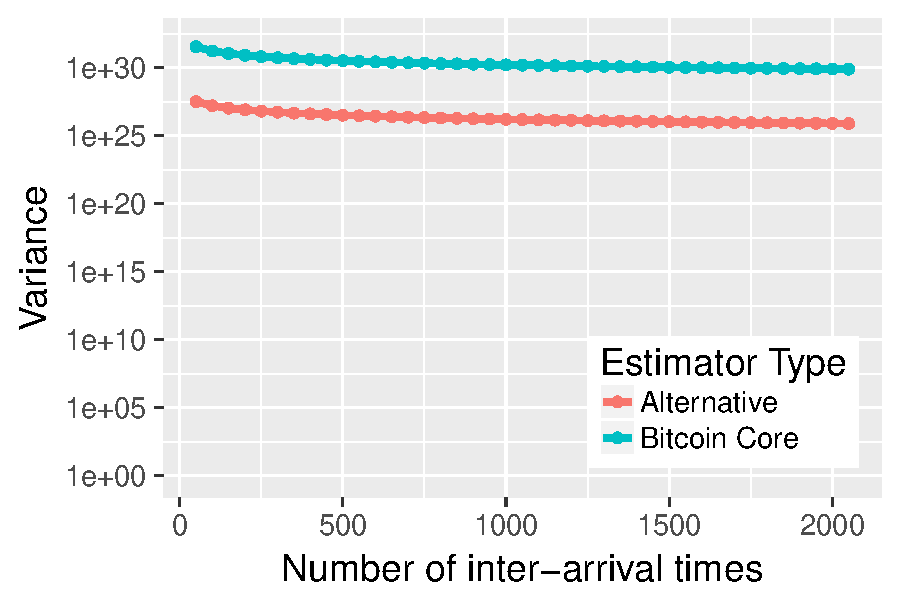
\includegraphics[width=\textwidth]{graphs/variance}
        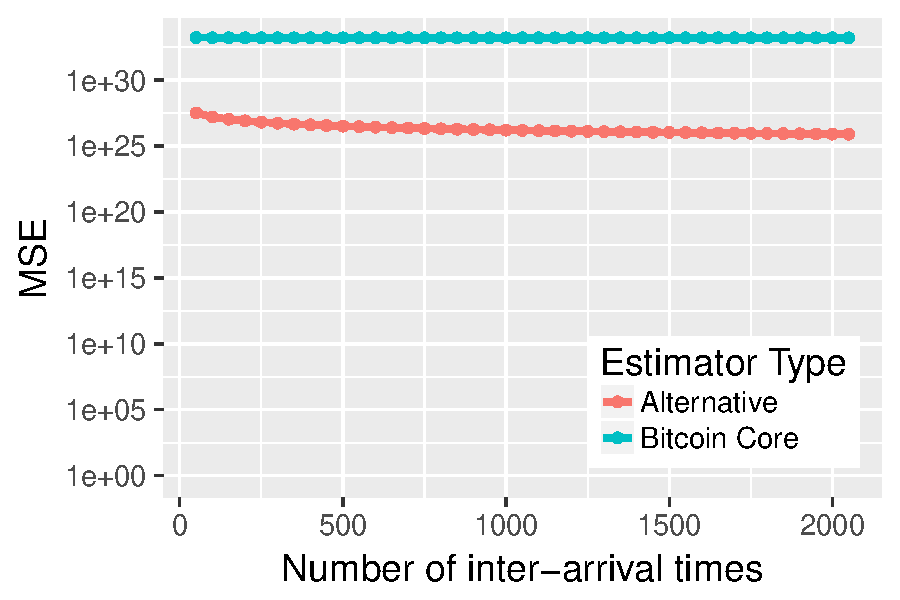
\includegraphics[width=\textwidth]{graphs/MSE}
    \end{minipage}  
    \caption{Variance (top) and mean squared error (bottom) of the difficulty algorithm of Bitcoin Core and our estimator, as the number of inter-arrival times increases. Note that the $y$-axis is in log scale.}
    \label{fig:MSE}
\end{figure}

%\begin{figure}
%  \hspace{-1cm}
%    \begin{minipage}[b]{0.55\textwidth}
%        %\centering
%        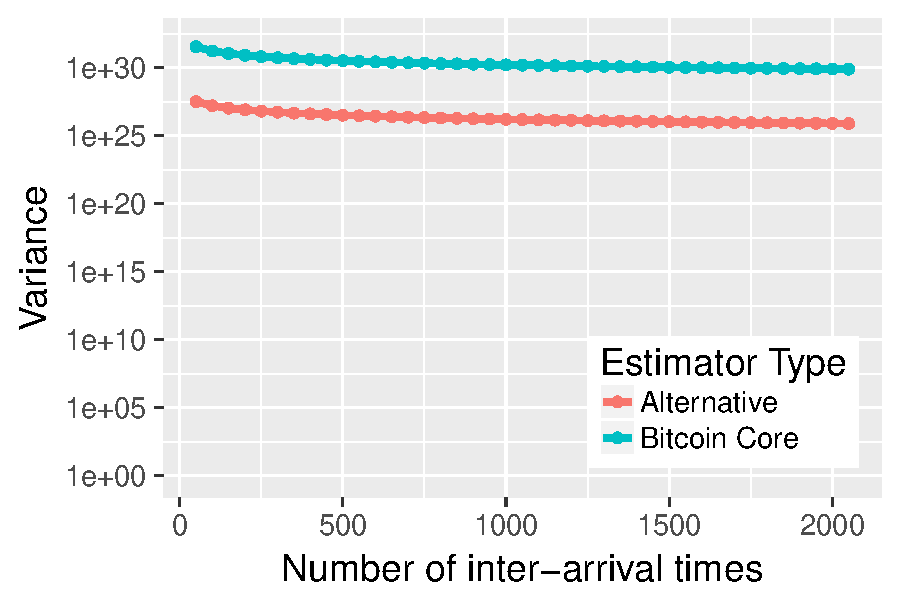
\includegraphics[width=\textwidth]{graphs/variance}
%    \end{minipage}
%    \begin{minipage}[b]{0.55\textwidth}
%        %\centering
%        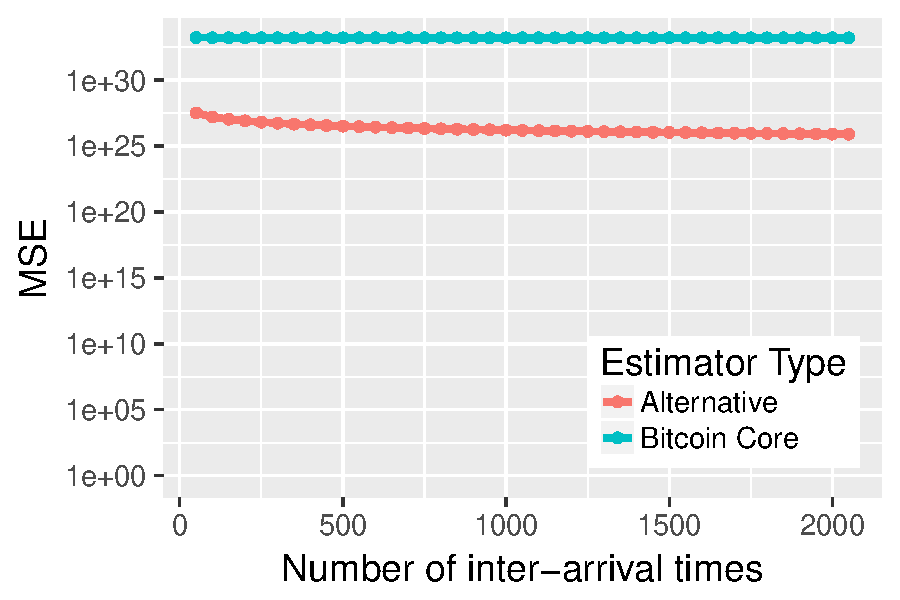
\includegraphics[width=\textwidth]{graphs/MSE}
%    \end{minipage}  
%    \caption{Variance (left) and mean squared error (right) of the difficulty algorithm of Bitcoin Core and our estimator, as the number of inter-arrival times increases. Note that the $y$-axis is in log scale.}
%    \label{fig:MSE}
%\end{figure}

%%%%%%%%%%%%%%%%%%%%%%%%%%%%%%%%%%%%%%%%
\section{Proposed Work} \label{section:difficulty-proposed-work}
In this section, we introduce status reports that are to be used for a second estimator, and then we discuss future work.

\subsection{Status Reports}
Attackers can easily lie about the timestamps on the blocks with our new time based estimator. Therefore, an alternative estimator we plan to develop uses status reports, which is a block header except that the POW does not satisfy the current target. Every $\alpha$ minutes, a parameter determined by the network, the miners send periodic status reports that include the minimum hash value, which represents the hash found since the last block broadcast on the chain. These reports add no computational load to miners, and are stored neither on the blockchain nor at peers that receive them past their usefulness. They are small and can be broadcast out-of-band, for example via RSS or Twitter. Just like block headers, reports are verifiable as authentic POW by third parties. To be clear, each status report does not directly report the minimum hash value; instead, reports are of the input values to the POW algorithm. Because attackers can't lie about their POW, an estimator based on the minimum hash value is safer and can be used to adjust the emergency difficulty when the network fails to produce a block for an unusually long time. We plan to compute the the variance and MSE of the status report based estimator, and compare its performance with other methods.

\subsection{Key Questions}
We were able to show that our time based estimator performs better than Bitcoin Core's unjustified method. To extend this chapter, we propose to answer the following questions centered around a few key themes:
\begin{enumerate}
\item \textbf{Analysis of attacks against our estimators.} What happens when the timestamps on the blocks are reported inaccurately by an attacker? How much error can an attacker introduce?
\item \textbf{Security bounds of the estimators.} What are the Chernoff bounds associated with our estimators?
\item \textbf{Settings of network parameters and their consequences.} How often should difficulty be adjusted? How often should miners send status reports? Should non-overlapping windows of blocks be used to compute difficulty at each iteration? Should there be some overlap of blocks between windows at each iteration?
\item \textbf{Individual parameter settings for peers.} Given a required error rate, what is the shortest window of time (or number of blocks) needed to estimate difficulty correctly?
\item \textbf{Fluctuations in mining power.} Given that mining power is changing, how quickly can either estimator adapt to change?
\item \textbf{Pros and cons of our estimators.} What are the advantages and disadvantages of status reports compared to the time based estimator? For example, the status report based estimator uses the minimum hash value, which is arguably safer because miners have to show their POW. On the other hand, the time based estimator can be utilized without additional functionality to Bitcoin Core.
\end{enumerate}

%\paragraph*{Overview}

%\begin{equation}
%\arg\max_\mathbf{s} p(\mathbf{s}|u).
%\end{equation}
%
%\begin{figure}\begin{center}
%		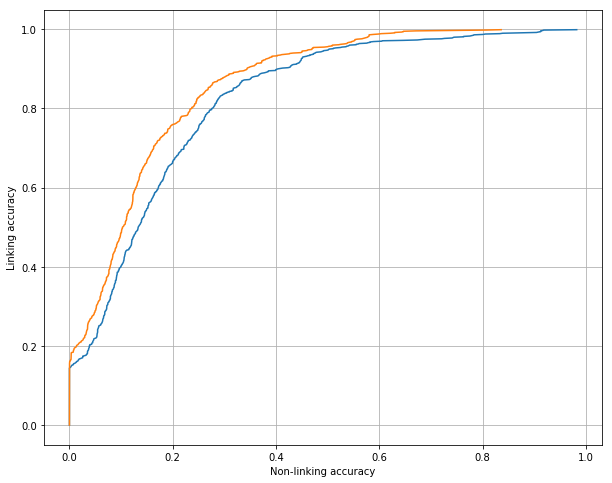
\includegraphics[width=0.7\textwidth]{graphics/linking2}
%		\caption{The $x$-axis represents accuracy of identifying a set of traces unlinked, and the $y$-axis represents the accuracy of the same set linked based on Equation~\ref{eq:link3}. Red is a link before, and blue is a link after.
%		\label{fig:linkcdf}}
%\end{center}\end{figure}
%!TEX root = umthsmpl.tex
\chapter{Graphene: Efficient Block Announcements}
\label{graphene}

\section{Background}
In this section, we describe the signaling mechanism behind blockchain systems, explain the operation of IBLTs and summarize related work.

%%%%%%%%%%%%%%%%%%%%%%%%%%%%%%%%%%%%%%%%%%%%%%%
\subsection{Topology and Signaling in Blockchain Systems} 
Bitcoin propagates new transaction and
block announcements by flooding throughout a p2p random graph of full
nodes and miners. Each peer in the graph requests direct connections
to 8 other peers, and accepts requests for connections from up to 117
other peers. A peer will offer a newly created transaction to each
neighbor via an {\tt inv} message, which reports the hash of the
transaction content as its ID. If a peer does not already possess the
transaction, it will request it using a {\tt getdata} message. Blocks
are handled similarly: {\tt inv} messages describe a block by its ID, which
is created from the hash of the block's contents.  Upon receiving the
{\tt inv}, peers will request the block if they do not already have it.
Hence, in today's topology, {\tt inv} messages cross every edge in the
random graph once, while the actual transaction and block data
typically propagate along only a spanning tree of the graph (more
edges will be traversed if there are propagation delays).  For
convenience, we refer to the set of (unconfirmed)
transaction IDs that a peer knows about as the {\em IDpool}. Actual
transaction contents are placed in the mempool.

%%%%%%%%%%%%%%%%%%%%%%%%%%%%%%%%%%%%%%%%%%%%%%%
\subsection{Related Work} 
The main limitation we are addressing with Graphene is the inefficiency of blockchain systems in disseminating block data.  A block announcement
must be validated using  the transaction content comprising the block.  However, it is likely that the majority of the
peers have already received these transactions, and they only
need to discern them from those in their
mempool. Additionally, in Section~\ref{section:difficulty-proposed-work}, we propose using status reports, blocks announcement that do not satisfy the difficulty requirement of the network, for the emergency difficulty algorithm. Therefore, on top standard blocks, we are proposing to add more network traffic, requiring an even more efficient method of block propagation.

In principle, a block announcement needs to include only the IDs of those transactions,
and accordingly, Corallo's {\em Compact Block} design~\cite{Corallo:2016} --- which has been recently deployed --- significantly reduces block size by including a  transaction ID list at the cost of increasing coordination to 3 roundtrip times.
%After the block's {\tt inv} has been sent, the receiver requests the block. The sender sends the IDs of transactions (in fact, just the first 5 bytes of each). The receiver then requests the contents of any transaction if previously unseen.
%
{\em Xtreme Thinblocks}~\cite{Tschipper:2016}, an alternative protocol, works similarly to Compact Blocks but has greater data overhead. Specifically, after receiving an {\tt inv} for a
 block, the receiver creates a Bloom filter of her mempool with FPR
 $f=1/n$, where $n$ is the number of transactions in the block. The
 sender then sends a \textit{thinblock transaction} that contains
 block header information, all transaction IDs in the block and any
 transactions that do not pass through the Bloom filter, enabling the
 receiver to recreate the block.
 As a result, Xtreme Thinblocks are larger than Compact Blocks but require just 2 roundtrip times. Relatedly, the community has discussed in forums the use of IBLTs (alone) for reducing block announcements\cite{andresen:2014,Russel:2014}, but these schemes have not been formally evaluated and are less efficient than our approach. Our novel method, which we prove and demonstrate is smaller than all of these recent works, requires just 2 roundtrip times for coordination.

%%%%%%%%%%%%%%%%%%%%%%%%%%%%%%%%%%%%%%%%%%%%%%%
 \subsection{Overview of IBLTs}
We make use of Invertible Bloom Lookup Tables (IBLTs)~\cite{goodrich:2011}, which is an efficient data structure  for {\em set reconciliation} between two peers.  Like 
  Bloom filters~\cite{Bloom:1970}, IBLTs allow
  two parties to determine, with high probability, which values from a
  set they share in common.  But unlike Bloom filters, IBLTs enable the
  recovery of any missing values, which are assumed to be of fixed
  size and encoded as binary strings.  Key-value pairs can be
  inserted, retrieved and deleted like an ordinary hash table.  An
  IBLT consists of $m$ entries, each storing a \texttt{count}, a
  \texttt{keySum}, and a \texttt{valueSum}, all initialized to zero. 
  
  A new value $v$ is inserted into location $i=h(v)$ based on
the hash of its value such that $i < m$.  At entry $i$, all three
fields are incremented or xored. In particular, standard
addition is used for the \texttt{count} field, but \texttt{xor} is
used to add to the \texttt{keySum} and \texttt{valueSum} fields. An
item can be deleted similarly: at the correct entry, \texttt{count}
is subtracted by 1, and the \texttt{valueSum} and \texttt{keySum}
fields are \texttt{xor}'ed.  When $\mbox{\texttt{count}} \equiv 1$
the \texttt{valueSum} field contains the actual value of the sole
item remaining in the cell.  (The purpose of the \texttt{keySum}
field is to support a $\texttt{GET}()$ operation for a given
key: that is, if $\mbox{\texttt{count}} \equiv 1$ and
$\texttt{keySum} \equiv h(v)$, then
$\texttt{valueSum} \equiv v$.)
IBLTs use $k > 1$ hash functions to store each value in $k$ entries, which we collectively call a value's \emph{entry set}.  
If table space is sufficient, then with high probability for at least one of the $k$
entries, $\texttt{count} \equiv 1$.
%, and so \texttt{keySum} and \texttt{valueSum} fields are recoverable~\cite{goodrich:2011}.

Suppose that two peers each have a list of values, $V$ and $V'$,
respectively, such that the difference is expected to be small.  The
first peer constructs an IBLT $L$ (with $m$ entries) from $V$.  The
second peer constructs $V'$ from $L'$ (also having $m$ entries).
Eppstein et al.~\cite{eppstein:2011} showed that a cell-by-cell
difference operator can be used to efficiently compute the symmetric
difference $L \bigtriangleup L'$.  For each pair of fields $(f, f')$,
at each entry in $L$ and $L'$, we compute either $f \oplus f'$ or
\mbox{$f - f'$} depending on the field type.  When
$|\mbox{\texttt{count}}| \equiv 1$ at any entry, the corresponding
value can be recovered.  
% If $\mbox{\texttt{count}} \equiv 1$, then the value belongs to
% $L \setminus L'$.  And if $\mbox{\texttt{count}} \equiv -1$, then
% the value belongs to $L' \setminus L$.
  Peers proceed by removing the recoverable key-value pair from all entries in the value's entry set.
%all values corresponding to these unit counts---not only from the
%recoverable entry, but also from all entries in the value's entry set.
This process will generally produce new recoverable entries, and
continues until nothing is recoverable.
 
%%%%%%%%%%%%%%%%%%%%%%%%%%%%%%%%%%%%%%%%%%%%%%%
\section{Graphene}

In this section, we detail \emph{Graphene},
%(i.e., the pending transactions they may
%contain). 
where a receiver 
learns the set of specific transaction IDs that are contained in a
(pending or confirmed) block containing $n$ transactions. Unlike other approaches, Graphene never  sends an explicit list of transaction IDs, instead it sends  a small Bloom filter and a very small IBLT.  

%!TEX root = canary.tex

{ \relsize{-1.25}
\begin{myprot}{\textbf{\Mf}}
\label{protocol:pblt}
\STATE \sender Sends \textit{inv} for a block.
%
\STATE \recvr \hspace{-.1mm}Requests unknown block; includes count of txns in her IDpool, $m$.
\STATE \sender  Sends Bloom filter \S and IBLT \I (each created from the set of $n$ txn IDs in the block) and essential Bitcoin header fields.  The FPR of the filter is $f=\frac{a}{m-n}$, where $a=n/(c\tau)$.% $a$ is determined by Eq.~\ref{eq:min.a}.
%
\STATE \recvr Creates IBLT $\cal{I}'$ from the txn IDs that pass through $\cal{S}$. She decodes the {\em subtraction}~\cite{eppstein:2011} of the two blocks, $\cal{I} \bigtriangleup \cal{I'}$.\end{myprot}
}


%%%%%%%%%%%%%%%%%%%%%%%%%%%%%%%%%%%%%%%%%%%%%%%
\subsection{The Protocol}
The intuition behind Graphene is as follows. The sender creates an IBLT \I
from the set of transaction (txn) IDs in the block. To help the receiver
create the same (or similar) IBLT, he also creates a Bloom filter \S
 of the transaction IDs in the block. The receiver uses \S to filter out
transaction IDs from her IDpool %pool of received transaction IDs (which we call the ) 
and creates her own IBLT $\cal{I}'$. She then attempts to use \Ip to \emph{decode} $\cal{I}$, which, if successful, will yield
the transaction IDs comprising the block. The number of transactions
that falsely appear to be in $\cal{S}$, and therefore are wrongly added to
$\cal{I}'$, is determined by a parameter controlled by the sender. Using
this parameter, he can
create \I such that it will decode with very high probability.  

A Bloom filter is an array of $x$ bits
representing $y$ items.  Initially, the $x$ bits are cleared. Whenever
an item is added to the filter, $k$ bits, selected using $k$ hash functions, in the bit-array are set. The number of bits
required by the filter is $x =\sfrac{-y\ln(f)}{\ln^2(2)}$, where $f$ is
the intended false positive rate (FPR).  For Graphene, we set $f=a/(m-n)$,
where $a$ is the expected difference between \I and \Ip .
Since the Bloom filter contains $n$ entries, and we need to convert to
bytes, its size is 
$$\frac{-\ln(\frac{a}{m-n})}{\ln^2(2)}\frac18. $$

It is also the case that $a$ is the primary parameter of the IBLT
size.  IBLT \I can be decoded by IBLT \Ip with very high probability
if the number of cells in \I is $d$-times the expected symmetric
difference between the list of entries in \I and the list of entries
in $\cal{I}'$. In our case, the expected difference is $a$, and we set
$d=1.5$ (see Eppstein et al.~\cite{eppstein:2011}, which explores
settings of $d$). Each cell in an IBLT has a {\tt count}, {\tt keySum} and
{\tt valueSum}.
%{\em count}, a {\em hash}
%value, and a stored {\em value}.  
(It can also have a key, but we have
no need for a key). For us, the count field is 2 bytes, the
keySum is 4 bytes, and the valueSum is the last 5 bytes of the
transaction ID (which is sufficient to prevent collisions). In sum,
the size of the IBLT with a symmetric difference of $a$ entries is
$1.5(2+4+5)a=16.5a$ bytes.
Thus, the total cost in bytes, $T$, for the Bloom filter and IBLT are
given by 
$$T(a)= n\frac{-\ln(f)}{c}+ a\tau = n\frac{-\ln(\frac{a}{m-\mu})}{c}+ a\tau,$$ 
where all Bloom filter constants are grouped together as
$c=8\ln^2(2)$, and we let the overhead on IBLT entries be the constant
$\tau=16.5$.

To set the Bloom filter as small as possible, we must ensure
that the FPR of the filter is as high as permitted. If we assume 
that all {\tt inv} messages are sent ahead of a block, we know that the receiver already has all
of the transactions in the block in her IDpool (they need not be in her mempool). 
%We
%enforce a rule in Graphene that all {\tt inv} messages are sent ahead of a block
%announcement, and thus, can assume that the receiver already has all
%of the transactions in the block in her IDpool (they need not be in her mempool). 
Thus, $\mu=n$; i.e.,  we allow for $a$ of $m-n$ transactions
to become false positives, since all transactions in the block are
already guaranteed to pass through the filter. It follows that
\begin{align}
T(a) = n\frac{-\ln(\frac{a}{m-n})}{c}+ a\tau.~\label{eq:tcost}
\end{align}
Taking the derivative w.r.t.\ $a$, Eq.~\ref{eq:tcost} is
minimized\footnote{Actual implementations of Bloom filters and IBLTs
  involve several (non-continuous) ceiling functions such that we can re-write:
\vspace{-2ex}
\begin{align}
T(a) =& \left(\lceil\ln(\frac{m-n}{a})\rceil\left\lceil  \frac{n\ln(\frac{m-n}{a})}{\lceil\ln(\frac{m-n}{a})\rceil\ln^2(2)} \right\rceil\right)\frac18 + \lceil a\rceil\tau.\label{eq:ceiling-TA}
\end{align}
The optimal value of Eq.~\ref{eq:ceiling-TA} can be found with a simple brute force
loop.  We compared the value of $a$ picked by using 
$a=n/(c\tau)$ to the cost for that $a$ from Eq.~\ref{eq:ceiling-TA}, for valid combinations of $50\leq n \leq 2000$
and $50\leq m \leq 10000$. We found that it is always within 37\% of
the cost of the optimal value from Eq.~\ref{eq:ceiling-TA}, with a median difference of 16\%. In
practice, a for-loop brute-force search for the lowest value of $a$ is
almost no cost to perform, and we do so in our simulations.}
 when when $a=n/(c\tau)$.

%Because Bloom filters are randomized data structures, $a$ of the $m-n$
%transactions that pass through the Bloom filter might not only be the
%transactions in the block, but also additional ones. Therefore, the
%The Bloom filter serves an error correcting mechanism, enabling the
%receiver to correctly detect the false positive transactions that pass
%through the Bloom filter. 
Due to the randomized nature of an IBLT,
there is a non-zero chance that it will fail to decode. In that case,
the sender resends the IBLT with double the number of cells (which is
still very small). In our simulations, presented in the next section,
this doubling was sufficient for the incredibly  few IBLTs that 
failed.

{\begin{myprot}{\textbf{CompactBlocks}}
\label{protocol:compact}
\STATE \sender Sends {\tt inv} for a block that has $n$ txns.
\STATE \recvr If block is not in mempool, requests compact block.
\STATE \sender Sends the block header information, all txn IDs in the block and any full txns he predicts the sender hasn't received yet.
\STATE \recvr Recreates the block and requests missing txns if there exist any.
\end{myprot}}

%%%%%%%%%%%%%%%%%%%%%%%%%%%%%%%%%%%%%%%%%%%%%%%
\subsection{Comparison to Compact Blocks} 
Compact Blocks\cite{Corallo:2016} is to our knowledge the best-performing related work. It has several modes of operation, and 
%The receiver has the
%option of switching between three modes via a message to the sender:
%\textit{Legacy Relaying}, \textit{High Bandwidth Relaying} and
%\textit{Low Bandwidth Relaying}. 
we examined the \textit{Low Bandwidth
  Relaying} mode due to its bandwidth efficiency, which operates as follows. 
%The receiver sends a message indicating the mode she wants to communicate in. 
After fully
validating a new block, the sender sends an {\tt inv}, for which the receiver sends a {\tt getdata} message if she
doesn't have the block. The sender then sends a {\tt compact block}
that contains block header information, all  transaction IDs (shortened to 5 bytes)
in the block, and any transactions that he predicts the receiver does
not have (e.g., the coinbase). If the receiver still has missing transactions, she requests
them via an {\tt inv} message. Protocol~\ref{protocol:compact} outlines
this  mode of Compact Blocks. The main difference between Graphene and Compact Blocks is that instead of
sending a Bloom filter and an IBLT, the sender sends block header
information and all shortened transaction IDs to the receiver. 

A detailed example of how to calculate the size of each scheme is below; but we can state more generally the following result. For a
block of $n$ transactions, Compact Blocks costs $5n$ bytes. For both
protocols, the receiver needs the {\tt inv} messages for the set of
transactions in the block before the sender can send it. Therefore, we
expect the size of the IDpool of the receiver, $m$, to be constrained
such that $m \geq n$. Assuming that $m > 0$ and $n > 0$, the following
inequality must hold for Graphene to outperform Compact Blocks: 
\begin{eqnarray}
n\frac{-\ln(\frac{a}{m-n})}{c}+ a\tau &<& 5n\\
n&>& \frac{m}{1287670}.
\end{eqnarray}
In other words, Graphene is strictly more efficient than Compact Blocks {\em unless} the  set of unconfirmed transactions held by peers  is 1,287,670 times larger than the block size (e.g.,  over 22 billion unconfirmed transactions for the current block size.)  Finally, we note that Xtreme Thinblocks~\cite{Tschipper:2016} are  strictly larger than Compact Blocks since they contain all IDs and a Bloom filter, and therefore Graphene performs strictly better than Xtreme Thinblocks as well. 

\para{Example.} A receiver with an IDpool of $m=4000$ transactions
makes a request for a new block that has $n=2000$ transactions. The
value of $a$ that minimizes the cost is $a=n/(c\tau)=31.5$. The sender
creates a Bloom filter \S with $f=a/(m-n)=31.5/2000= 0.01577$,
with total size of $2000\times -ln(0.01577)/c=2.1$~KB.  The
sender also creates an IBLT with $a$ cells, totaling $16.5a=521B$. In
sum, a total of $2160B+521B=2.6$~KB bytes are sent.  The receiver
creates an IBLT of the same size, and using the technique introduced
in Eppstein et al.\cite{eppstein:2011}, the receiver subtracts one
IBLT from the other before decoding. In comparison, for a block of $n$ transactions, Compact Blocks costs $2000\times5B = 10$~KB, over 3 times the cost of Graphene. 

\para{Ordered blocks.} Graphene does not specify an order for transactions
in the blocks, and instead assumes that transactions are sorted by
ID. Bitcoin requires transactions depending on another transaction in
the same block to appear later, but a canonical ordering is easy to
specify. If a miner would like to order transactions with some
proprietary method (e.g.,\cite{Hanke:2016}), that ordering would be
sent alongside the IBLT. For a block of $n$ items, in the worst case,
the list will be $n\log_2(n)$ bits long.  Even with this extra data, our approach is much more efficient than Compact Blocks.   In terms of the example above, if Graphene was to impose an ordering, the additional cost for $n=2000$ transactions would be $n \log_2(n)$ bits $= 2000\times log_2(2000)$ bits $= 2.74$~KB. This increases the cost of Graphene to $5.34$~KB, still almost half of Compact Blocks.

%In the next section, we show the results of hundreds of simulations of
%the full \bc system. In all trials, Compact Blocks are vastly more
%expensive than Graphene.

%In Section~\ref{sec:eval}, we provide specific empirical results from network simulation, where we use real IBLTs and Bloom filters to evaluate Graphene and Compact Blocks.

\subsection{Empirical Evaluation}



%!TEX root = umthsmpl.tex
\chapter{Reinforcement Learning Applied to Blockchain Systems}\label{selfishRL}
The hash rate of miners is the primary quantitative factor that determines the security of any POW based blockchain consensus algorithm. Recent models on attacks against blockchain systems assume that the hash rate of honest and malicious miners is known. However, hash rate estimation in blockchain systems introduces error into these models. Next, we quantify the error associated with estimating the hash rate of miners on Bitcoin Core, and justify our reasoning for using Reinforcement Learning (RL) methods.

\section{Hash Rate Estimation}
Given target $T_i$, the expected number of hashes, $h$, needed to meet the target for a block is
\begin{align}
\EX[h] = \frac{2^{256}-1}{T_i}.
\end{align}
$\EX[h]$ describes the \textit{total} number of expected hashes needed to find a block. We have observations regarding the \textit{time} it takes to generate a block. Let $X = X_1, \dots, X_{n}$, where $X \sim$ Exp$(\beta)$ with $\beta = 1/\lambda$. Note that in this scenario, $X$ is a random variable representing the inter-arrival time of blocks discovered by a {\em single miner}. We could also estimate the network-wide hash rate if we used {\em all} blocks instead of those by a specific miner. In Section~\ref{sec:time based} we have shown that the unbiased MLE estimator for $\beta$ is equation~\ref{eq:beta-hat}. Let $r$ be the miner's hash rate in minutes (i.e., the number of hashes per time unit), and $X = X_1, \dots, X_{n}$, where $X \sim$ Exp$(\beta)$, where $\beta = 1/\lambda$. We can use our estimate, $\hat{\beta}$, of $\beta$ to calculate a given miner's hash rate.
%Note that $\lambda r$ is the expected number of hashes each time a block is created 
\begin{align}
\EX[h] = r \lambda &= r \frac{1}{\beta}  \\
r &= \EX[h] \hat{\beta}
\end{align}
A miner's estimated hash rate 
given target $T_i$ and $n$ inter-arrival times for $n+1$ blocks discovered by that miner is 
\begin{align}
\frac{(2^{256}-1)\hat{\beta}}{T_i}.
\end{align}
%\para{Expected Value of Hash Rate.}
%\begin{align}
%\EX[r|T_i,X_1,...,X_n] &= \EX\bigg[\frac{(2^{256}-1)\hat{\beta}}{T_i}\bigg] \\
%&= \frac{(2^{256}-1)}{T_i}\EX[\hat{\beta}] \\
%&= \frac{(2^{256}-1)\beta}{T_i}
%\end{align}
%
%\para{Variance of Hash Rate.}
The variance associated with this estimate is
\begin{align}
\text{Var}(r|T_i,X_1,...,X_n) &= \text{Var}\bigg(\frac{(2^{256}-1)\hat{\beta}}{T_i}\bigg) \\
&= \frac{(2^{256}-1)^2}{T_i^2} \text{Var}(\hat{\beta}) \\
&= \frac{(2^{256}-1)^2\beta^2}{T_i^2n}.
\end{align}

%\para{Bias of Hash Rate.}
%\begin{align}
%\text{bias}(r|T_i,X_1,...,X_n) &= \EX[r|T_i,X_1,...,X_n] - r \\
%&= \frac{(2^{256}-1)\beta}{T_i} - \frac{(2^{256}-1)\beta}{T_i} \\
%&= 0
%\end{align}

\para{Example.}
The current Bitcoin Core difficulty, $D_i$, is $1,590,896,927,258 \approx 2^{40}$. Therefore, the current target, $T_i$, is
\begin{align}
T_i &= \frac{2^{224}}{D_i} = \frac{2^{224}}{2^{40}} \\
&\approx 2^{184}.
\end{align}
Then the variance associated with hash rate estimation approximately is
\begin{align}
\text{Var}(r|T_i,X_1,...,X_n) &= \frac{(2^{256}-1)^2\beta^2}{T_i^2n} \\
&\approx  \frac{(2^{256})^2\beta^2}{T_i^2n} \\
&\approx  \frac{(2^{256})^2\beta^2}{(2^{184})^2n} \\
&\approx  \frac{2^{512}\beta^2}{2^{368}n} \\
&\approx  2^{144}\frac{\beta^2}{n}.
\end{align}
The variance associated with estimating hash rate for $0 \leq \beta \leq 1$ and for any $n \in \mathbb{Z}^+ $ is large. We need more blocks than those that are on the Bitcoin Core blockchain to reduce variance. RL provides a solution to this problem because it assumes that an agents acts in an environment where there is uncertainty. Therefore, we use RL methods to search for the optimal strategies for an attacker, who wants to perform attacks on blockchain networks. Then we compare the optimal policy found by RL algorithms to those cited in previous work.

\section{Background}
In this section, we describe double spend and selfish mining attacks on blockchain systems, and explain the paradigms used to analyze these attacks.

\subsection{Double Spending} 
%A fundamental attack against Bitcoin is the 
{\em Double spend} attacks~\cite{Nakamoto:2009} work as follows. An attacker creates a transaction that moves
funds to a merchant's address. After the transaction appears in the
newest block on the main branch, the attacker takes possession of the purchased
goods. Using his mining power, the attacker then immediately releases
two blocks, with a transaction in the first that moves the funds to a
second attacker-owned address. Now the attacker has the goods and his
coin back. To defend against the attack, a merchant can refuse to
release goods to a customer until $z$ blocks have been
added to the blockchain including the first block containing a
transaction moving coin to the merchant's address.  Nakamoto
calculated the probability of the attack succeeding assuming that the
miner controlled a given fraction of the mining power~\cite{Nakamoto:2009};
for a given fraction, the probability of success decreases exponentially as $z$
increases. 

In general, a merchant may wait $z$ blocks before releasing goods,
which can thwart an attacker.
But choosing the minimum value of $z$ that secures a transaction is an
unresolved issue. The core Bitcoin client shows that a transaction is
unconfirmed until it is 6 blocks deep in the
blockchain\cite{bitcoin:confirmation}, and   advice from others is necessarily vague; e.g., ``for very large transactions, coin
owners might want to wait for a larger number of block
confirmations''~\cite{Bonneau:2015a}.   

%Blockchain systems~\cite{Nakamoto:2009} provide probabilistic consensus~\cite{Vukolic:2015} among a set of peers on the order and validity of a set of blocks, each containing transactions. The blockchain encodes the consensus as the {\em main chain} among all possible forks. 
%As the {\em depth} of a block on the main chain increases, there is an exponentially decreasing probability that network consensus will switch the main chain to a fork that does not include the block~\cite{Nakamoto:2009,Feller:1968}. This result assumes that the attacker never stops mining on the alternative fork, regardless of cost.  A more realistic model assumes that attackers have finite  time and resources, and would not expend resources on an attack that isn't expected to be profitable. 
%Furthermore, only in theory do blockchains accept new forks of any length from  attackers;  in practice, the largest attacks on blockchains have been manually set aside~\cite{Castillo:2016,Castillo:2016a,Gervais:2014}. 

Recently, Gervais et al.~\cite{Gervais:2016} evaluated the security of blockchains in terms of an attacker's economic profitably and assuming finite resources. They modeled a double-spending attacker's strategy  as a Markov Decision Process (MDP). MDPs are defined by a finite set of discrete states, a set of actions, a transition function, and a reward function. They defined each  state in the MDP as a tuple representing the following: the status of the fork, and the number of blocks mined by an attacker,  the number of blocks mined by the honest miners, and  the number of blocks mined by an {\em eclipse attack} victim~\cite{Heilman:2015}, respectively.   Gervais et al.\ encoded several factors into the MDP that affect  attacker strategy, including mining power, block depth, connectivity, and the impact of eclipse attacks. The MDP was implemented with a cutoff value of 20 blocks, representing an attack of finite duration. Using a search algorithm over the space defined by the MDP that simulates a blockchain system, they determined the maximum transaction value that would be safe from double spending by an economically rational attacker. This  approach is rich, capturing the optimal strategy for  double-spending (as well as selfish mining~\cite{eyal:2014,sapirshtein:2015}) given  network conditions and blockchain parameters.  Gervais et al.\ were able to reach interesting conclusions about the comparative performance and security of several widely used blockchains.

Sapirshtein et al.~\cite{sapirshtein:2015} first observed that some double-spend attacks can be carried out essentially cost-free in the presence of a concurrent selfish mining~\cite{eyal:2014} attack. 
More recent work extends the scope of double-spends that can benefit from selfish mining to cases where the attacker is capable of \emph{pre-mining} blocks on a secret branch at little or no opportunity cost~\cite{Sompolinsky:2016}. The papers identify the optimal mining strategy for an attacker and quantify the advantage he can expect to have over the merchant in terms of pre-mined blocks.
%This analysis is complementary to ours; it is possible to relatively easily incorporate the pre-mining advantage into our model by simply changing the attacker's block target from $z$ to $z-c$. We note that pre-mining in the context of the eclipse attack may not be feasible since an eclipse cannot generally be carried out for an indefinite period of time. Nevertheless, we intend to update both of our double-spend analyses to account for cost-free pre-mining in future work.

%Gervais et al.~\cite{Gervais:2016} is the work most directly related to our objectives.  Rosenfeld~\cite{Rosenfeld:2012} also has the same economic objective. As we discuss in Section~\ref{sec:discussion}, in general, the approach taken by past work, including Gervais et al., Rosenfeld, and the works cited above, models only the \emph{order} of block creation, which is a discrete process; they do not model block mining time, which is a continuous process. As a result, it is difficult to extend those results to model cost in circumstances where the attacker is given a specific deadline in time (as we have done in our eclipse attack analysis) or where an attacker drops out (because the honest miners have already won) but has spent time mining. We develop a richer, continuous-time model that explicitly accounts
%for attacker cost as a function of mining duration.  

\subsection{Selfish Mining}

The standard Bitcoin protocol requires miners to broadcast a block they mined immediately. However, in the case of {\em selfish mining}, a miner deliberately withholds transaction information. The motivation is to bifurcate the chain and waste the computational resources of the honest miners should the network decide to build on the attacker's chain. An attacker can't profit economically since the number of blocks that can be created by a miner depends on the fraction of the mining power he has. However, selfish mining discards the honest miners' blocks, by releasing an alternative chain that takes over the current longest chain. If a selfish mining attack is successful, the selfish miners own a higher fraction of the blocks on the main chain because some portion of the blocks created by the honest network go to waste.

Eyal et al.~\cite{eyal:2014} modeled selfish mining using a Markov chain. Then Sapirshtein et al.~\cite{sapirshtein:2015} created a more complex model using a Markov decision process (MDP) for selfish mining and computed the $\epsilon$-optimal policy that increases a selfish miner's revenue. Recently, Gervais et al.~\cite{Gervais:2016} incorporated additional parameters such as network conditions and Bitcoin settings into the MDP to study the affects of such parameters on the attacker's policy. %that affect  attacker strategy, including mining power, block depth, connectivity, and the impact of eclipse attacks.

\section{Preliminary Work}
Sapirshtein~\cite{sapirshtein:2015} and Gervais~\cite{Gervais:2016} use an {\em average reward} MDP for computing the optimal strategies for selfish mining and double-spending. Average reward MDPs, as the name suggests, maximize an agent's average return instead of {\em episodic} MDPs that maximize absolute return over time. In the following section, we formulate the problem as an episodic MDP that is more widely studied and easier to solve.

\subsection{Formulating the Problem as an Episodic MDP}
\para{States.} Using Sapirshtein et al.~\cite{sapirshtein:2015}'s model as a basis, we construct the following MDP that is a 6-tuple $\{S, A, P, R, \gamma, d_0\}$, where $S = \{(w, x, y, z, i, k)\}$ such that $w, x, y, z, i, k \in \mathbb{N}$. The state consists of a 6-tuple where each element represents the following: 1) $w$ is the number of blocks created by the honest miners on the main chain. 2) $x$ is the number of blocks created by the attacker. 3) $y$ is the number of attacker blocks that the honest network accepts as part of the main chain. 4) $z$ is a variable that represents the state of the main chain. If $z \equiv 1$, the attacker performed a {\tt match} action, resulting in a fork on the main chain. If $z \equiv 0$, the attacker mined the last block, and if $z \equiv 2$, the honest network mined the last block, enabling the attacker to release a competing block if he has any. 5) $i$ is the number of attacker blocks on the main chain so far. 6) $k$ is the {\em total} number of blocks on the main chain so far. Note that this representation assumes that all blocks build on the same parent block.

\para{Actions.} $A = \{\texttt{adopt}, \texttt{mine}, \texttt{override}, \texttt{match}\}$. \texttt{adopt} refers to the adoption of the main chain, thereby discarding all blocks created by the attacker (except those already accepted by the honest network). The action \texttt{mine} denotes that the attacker continues to mine, waiting to see who the next block will be discovered by. \texttt{override} refers to an attacker's releasing one more block than the honest miners' blocks on the main chain. This action can be viewed as honest or selfish depending on the current state. If the honest miners have no blocks on the main chain, an addition of a block to the main chain means that the attacker is honest. However, if the honest miners already have blocks on the main chain and the attacker releases an alternative chain that is 1 block longer than that created by the honest miners, then the attacker overwrites the main chain, wasting the victim's computational resources. The \texttt{match} action means that the attacker releases as many blocks as there are on the main chain, causing a bifurcation.

\para{Initial state distribution.} $d_0 = \{(0, 0, 0, 0, 0, 0)\}$, where $P(S_0 = (0, 0, 0, 0, 0, 0)) = 1$. In other words, the start state assumes that no blocks have been mined yet. If the attacker chooses the action \texttt{adopt} and the length of the main chain is greater than some CUTOFF, the agent goes back to the start state.

\para{Transition Function.} We consider 3 of parameters of interest -- $q$, CUTOFF and $a$ -- included in Gervais et al.~\cite{Gervais:2016}'s model. At each time step, a new block is created by the network: with probability $q$, where $q$ is the mining power of the attacker, the attacker is the winner of a new block. The honest network discovers a block with probability $1-q$. Not all actions are available in every state. The attacker can always choose the \texttt{mine} and \texttt{adopt} actions. If the attacker chooses an {\tt adopt} action, he discards all blocks he has created on his alternative chain and accepts the blocks on the main chain created by the honest network should there exist any. Additionally, \texttt{override} and \texttt{match} are only available when the attacker has enough blocks and the last blocks has been mined by the honest network. At CUTOFF $= 75$, the length of the main chain is equal to or longer than 75 blocks, and we force the attacker to choose the \texttt{adopt} action in order to have episodic trials. Our third parameter, $a$, represents network connectivity. If there is a fork of same length on the main chain, fraction $a$ of the honest miners build on the attacker's alternative chain. We set $a=1$ to give advantage to the attacker, and to analyze if RL methods can learn to take advantage of the \texttt{match} action. Therefore, in our formulation, if the attacker matches the main chain with a fork of the same length, all honest miners build on the attacker's chain. 

\section{Proposed Work}\label{section:selfishRL-proposed-work}
I propose to complete the following tasks to extend this chapter:
\begin{enumerate}
\item Prove that the episodic MDP presented above is equivalent to Sapirshtein et al.~\cite{sapirshtein:2015}'s average reward MDP.
\item Evaluate Sapirshtein et al.~\cite{sapirshtein:2015}'s model where an agent first calculates the hash rate of the attacker using our estimator with the given variance and MSE.
\item Run RL algorithms such as Q-learning and SARSA on the MDP presented, where the 3 network parameters discussed above are not revealed to an agent.
\item Compare the performance of RL algorithms to previous work.
\item Evaluate RL algorithms and Sapirshtein et al.~\cite{sapirshtein:2015}'s model when the mining power of the network is fluctuating.
\end{enumerate}


%!TEX root = umthsmpl.tex
\chapter{Timeline}
\label{timeline}


%%
%% Beginning of back matter
\backmatter  %% <--- mandatory

%%
%% We don't support endnotes

%%
%% A bibliography is required.
\interlinepenalty=10000  % prevent split bibliography entries
\bibliographystyle{umassthesis}
\bibliography{umthsmpl}
\end{document}

%%% Local Variables: 
%%% mode: latex
%%% TeX-master: t
%%% End: 
